\documentclass[a4paper,12pt]{article}

\usepackage[a4paper,left=20mm,right=20mm,bottom=20mm,top=20mm]{geometry}

\usepackage{hyperref}
\usepackage{float}
\usepackage{color}
\usepackage[style=numeric]{biblatex}
\addbibresource{references.bib}
\usepackage{multirow}
\usepackage{makecell}
\usepackage{threeparttable}
\usepackage{bm}
\usepackage{mathtools, nccmath}
\usepackage{amsmath,amsfonts}
\usepackage{algorithmic}
\usepackage{algorithm}
\usepackage{array}
\usepackage[caption=false,font=scriptsize,labelfont=sf,textfont=sf]{subfig}
\usepackage{textcomp}
\usepackage{stfloats}
\usepackage{url}
\usepackage{verbatim}
\setlength{\parindent}{0em}
\setlength{\parskip}{0.5em}
\usepackage{graphicx}
\hyphenation{op-tical net-works semi-conduc-tor IEEE-Xplore}

\begin{document}

\title{Weekly Report}
\author{Zhenyu Zhou}
\maketitle

\section{Joint Finger Knuckle and Fingerprint Verification}
\subsection{RFN64-RSSSIM with Quadruplet Loss}
The quadruplet loss can increase inter-class variance and decrease  intra-class variance result in more robust cluster when compared to the triplet loss function. Because the loss used two hard margin for training, the second margin is weak margin when compared to the first hard margin. The second margin is to help the original triplet loss for lower intra-class variance. For getting the best hard margin of quadruplet loss, we have tested the matching performance under changed $\alpha$ and $\alpha$2 from the Table \ref{quadruplet}.

% Please add the following required packages to your document preamble:
% \usepackage{multirow}
\begin{table}[ht]
    \centering
    \caption{Matching performance with different quadruplet margin}
    \begin{tabular}{ccccccccc}
    \hline
    \multirow{2}{*}{Loss} & \multirow{2}{*}{$\alpha$} & \multirow{2}{*}{$\alpha$2} & \multicolumn{2}{c}{Left-Little}    & \multicolumn{2}{c}{Left-Ring}      & \multicolumn{2}{c}{Left-Index}     \\
                          &                         &                         & EER             & GAR              & EER             & GAR              & EER             & GAR              \\ \hline
    RSSSIM                & 0.5                     & 0.2                     & 4.25\%          & 83.00\%          & 0.83\%          & 96.00\%          & 2.67\%          & 85.50\%          \\
    \textbf{RSSSIM}       & \textbf{0.5}            & \textbf{0.3}            & \textbf{3.75\%} & \textbf{88.00\%} & \textbf{0.75\%} & \textbf{98.00\%} & \textbf{2.08\%} & \textbf{92.00\%} \\
    RSSSIM                & 0.5                     & 0.4                     & 4.53\%          & 87.00\%          & 1.08\%          & 97.00\%          & 2.58\%          & 92.00\%          \\
    RSSSIM                & 0.5                     & 0.5                     & 3.75\%          & 86.50\%          & 0.67\%          & 97.00\%          & 1.92\%          & 91.00\%          \\
    \textbf{RSSSIM}       & \textbf{0.6}            & \textbf{0.3}            & \textbf{4.45\%} & \textbf{88.50\%} & \textbf{0.67\%} & \textbf{97.50\%} & \textbf{1.92\%} & \textbf{94.00\%} \\
    RSSSIM                & 0.6                     & 0.4                     & 3.43\%          & 84.00\%          & 0.50\%          & 97.00\%          & 1.92\%          & 89.50\%          \\
    RSSSIM                & 0.6                     & 0.5                     & 4.00\%          & 68.00\%          & 0.50\%          & 89.50\%          & 2.00\%          & 84.00\%          \\
    RSSSIM                & 0.5                     & 0                       & 4.08\%          & 85.50\%          & 0.67\%          & 97.00\%          & 2.58\%          & 91.00\%          \\ \hline
    \end{tabular}
    \label{quadruplet}
\end{table}

From the above Table \ref{quadruplet}, we  can find two cases which was bolded can get the best finger knuckle matching performance on the little, ring, and index finger knuckle of left hand. Therefore, we use two of them to test finger knuckle matching performance on the rest finger knuckle from the Table \ref{quadruplet-best}. The performance of RSSSIM-0.5-0.3 and RSSSIM-0.6-0.3 are similar with each other, but the RSSIM-0.6-0.3 is slightly better than the RSSSIM-0.5-0.3.


% Please add the following required packages to your document preamble:
% \usepackage{multirow}
\begin{table}[ht]
    \centering
    \caption{Compare RSSSIM-0.5-0.3 and RSSSIM-0.6-0.3 matching performance}
    \begin{tabular}{cccc}
    \hline
    \multicolumn{2}{c}{Performance}     & RSSSIM-0.5-0.3 & RSSIM-0.6-0.3 \\ \hline
    \multirow{2}{*}{Left-Little}  & EER & 3.75\%         & 4.45\%        \\
                                  & GAR & 88.00\%        & 88.50\%       \\ \hline
    \multirow{2}{*}{Left-Ring}    & EER & 0.75\%         & 0.67\%        \\
                                  & GAR & 98.00\%        & 98.00\%       \\ \hline
    \multirow{2}{*}{Left-Index}   & EER & 2.08\%         & 1.92\%        \\
                                  & GAR & 92.00\%        & 92.00\%       \\ \hline
    \multirow{2}{*}{Left-Thumb}   & EER & 3.75\%         & 3.50\%        \\
                                  & GAR & 76.00\%        & 81.00\%       \\ \hline
    \multirow{2}{*}{Right-Thumb}  & EER & 2.25\%         & 2.58\%        \\
                                  & GAR & 82.00\%        & 90.50\%       \\ \hline
    \multirow{2}{*}{Right-Index}  & EER & 1.75\%         & 1.92\%        \\
                                  & GAR & 94.00\%        & 95.00\%       \\ \hline
    \multirow{2}{*}{Right-Middle} & EER & 1.58\%         & 1.58\%        \\
                                  & GAR & 97.00\%        & 98.00\%       \\ \hline
    \multirow{2}{*}{Right-Ring}   & EER & 1.17\%         & 1.08\%        \\
                                  & GAR & 97.50\%        & 98.00\%       \\ \hline
    \multirow{2}{*}{Right-Little} & EER & 6.00\%         & 5.39\%        \\
                                  & GAR & 84.00\%        & 83.00\%       \\ \hline
    \end{tabular}
    \label{quadruplet-best}
\end{table}


\subsection{Finger Knuckle and Fingerprint Score Fusion}
I have tried dynamic, holistic, and nonlinear fusion method to fusion finger knuckle matching score and fingerprint matching score. After comparing these three different fusion method, the performance of dynamic and holistic method are similar, and all of them are better than the nonlinear fusion method. As a result, the performance of holistic method is slightly better than the dynamic method, then I choose it to show the fusion performance as shown on the Fig. \ref{fusion-score}

\begin{figure}[ht!]
    \centering
    \subfloat[]{
        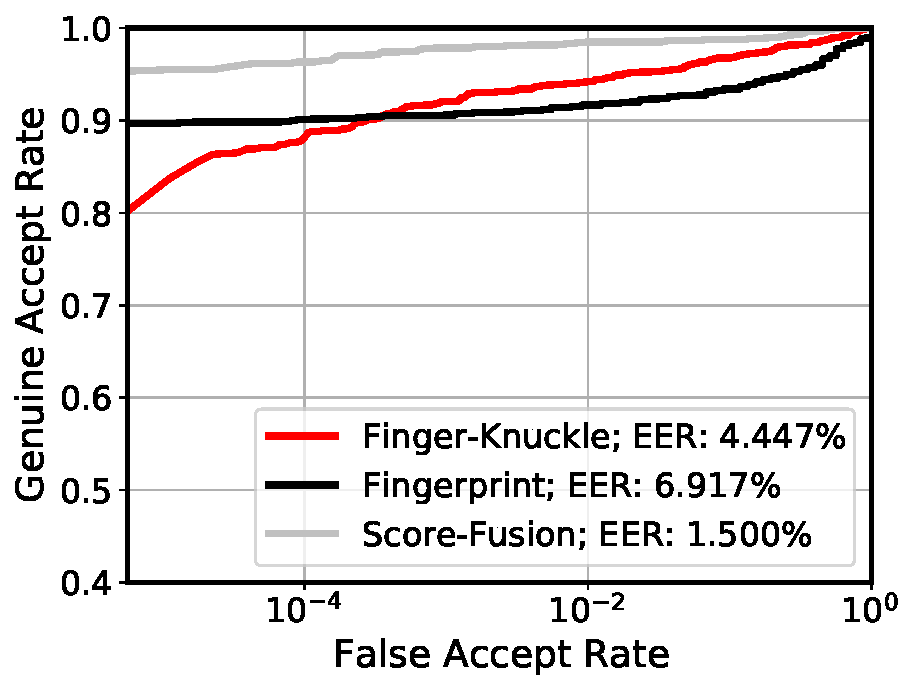
\includegraphics[width=2in]{Figure/09-12-2022/01(0.3-0.7).pdf}
        \label{}
    }
    \subfloat[]{
        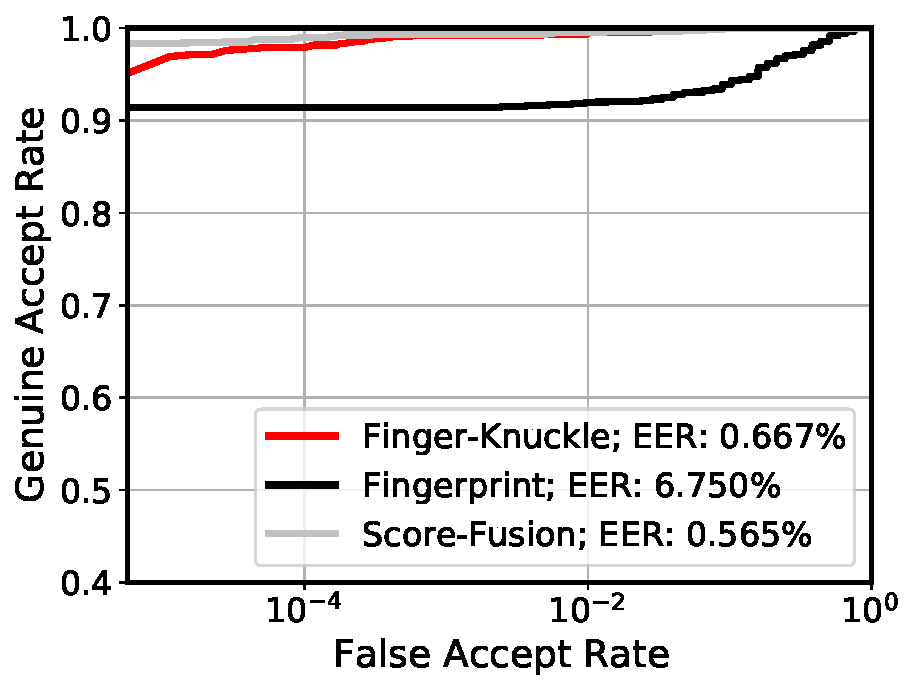
\includegraphics[width=2in]{Figure/09-12-2022/02(0.35-0.65).pdf}
        \label{}
    }
    \subfloat[]{
        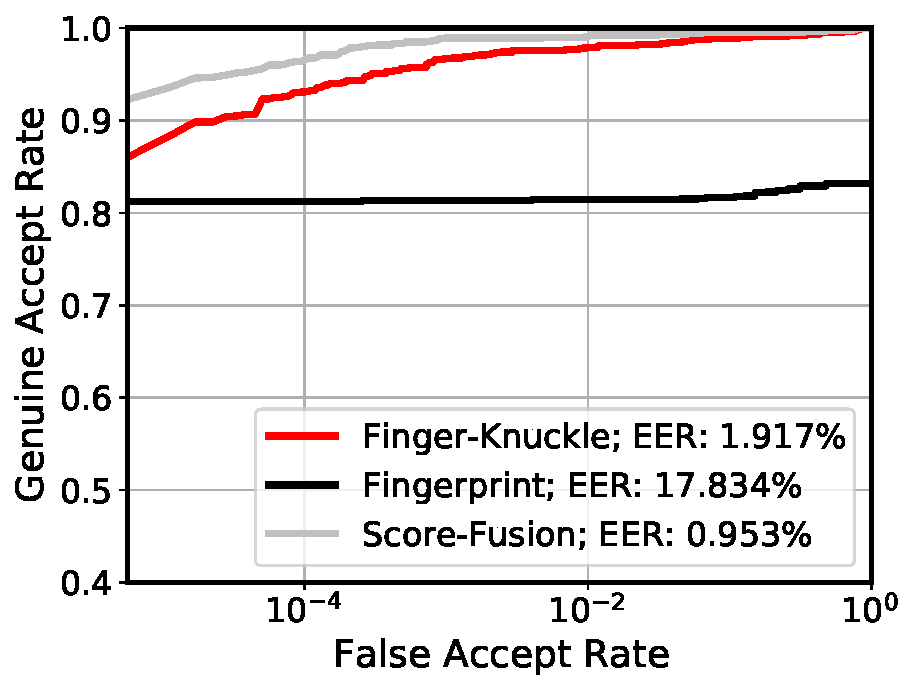
\includegraphics[width=2in]{Figure/09-12-2022/04(0.75-0.25).pdf}
        \label{}
    }

    \subfloat[]{
        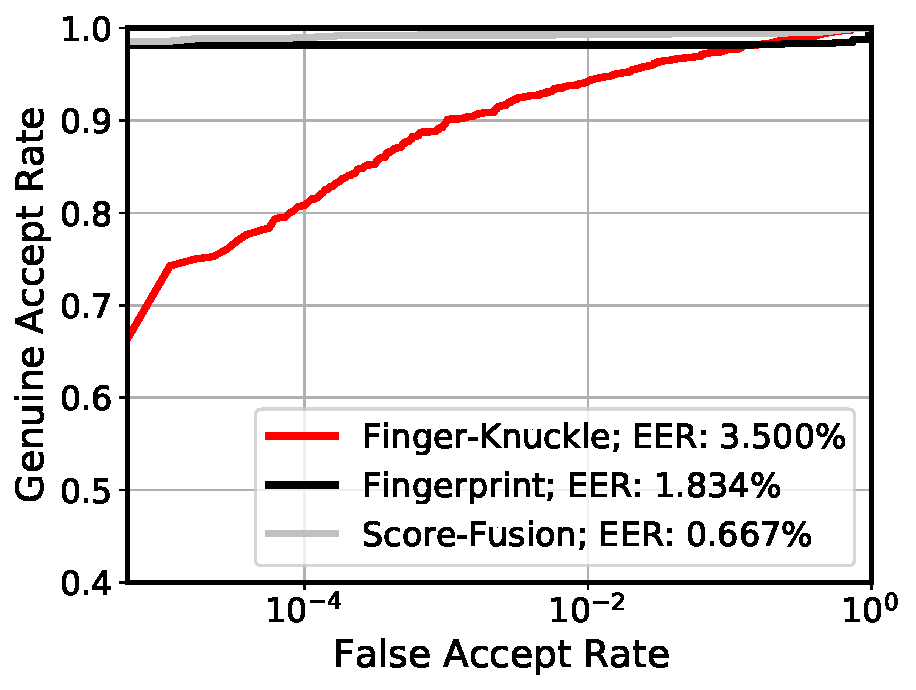
\includegraphics[width=2in]{Figure/09-12-2022/05(0.3-0.7).pdf}
        \label{}
    }
    \subfloat[]{
        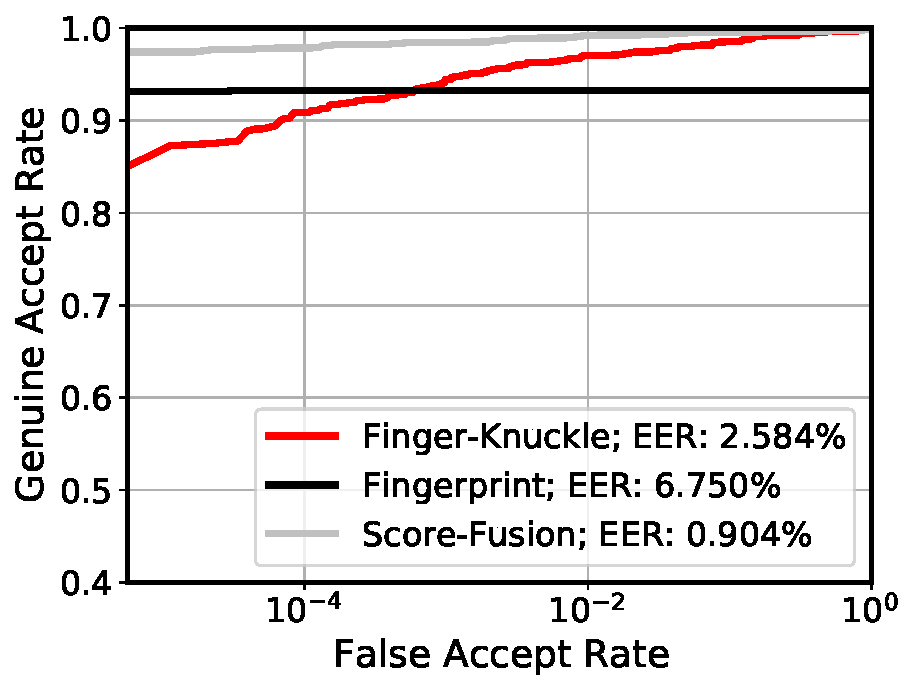
\includegraphics[width=2in]{Figure/09-12-2022/06(0.5-0.5).pdf}
        \label{}
    }
    \subfloat[]{
        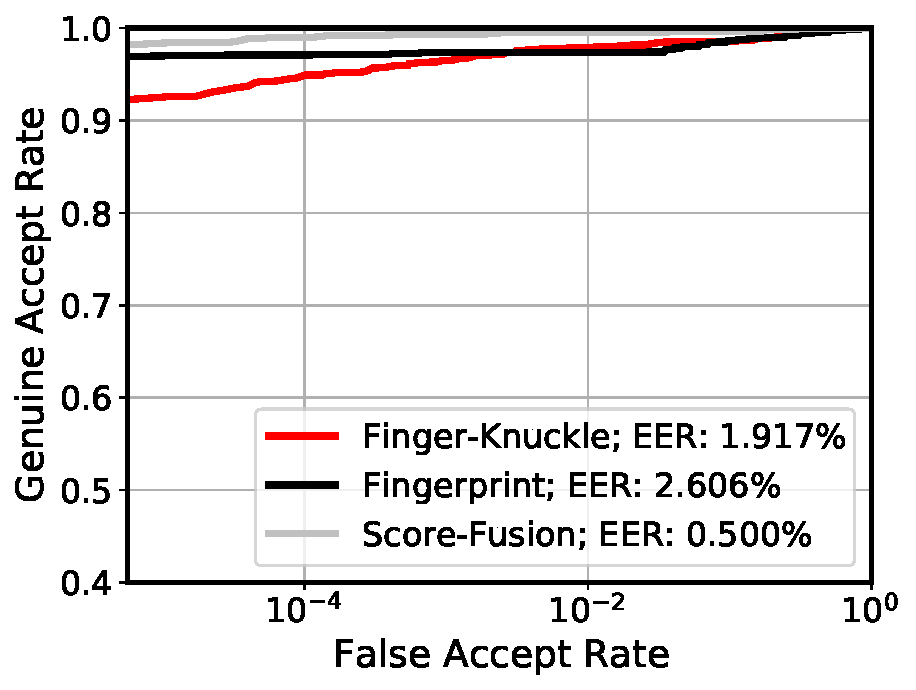
\includegraphics[width=2in]{Figure/09-12-2022/07(0.2-0.8).pdf}
        \label{}
    }

    \subfloat[]{
        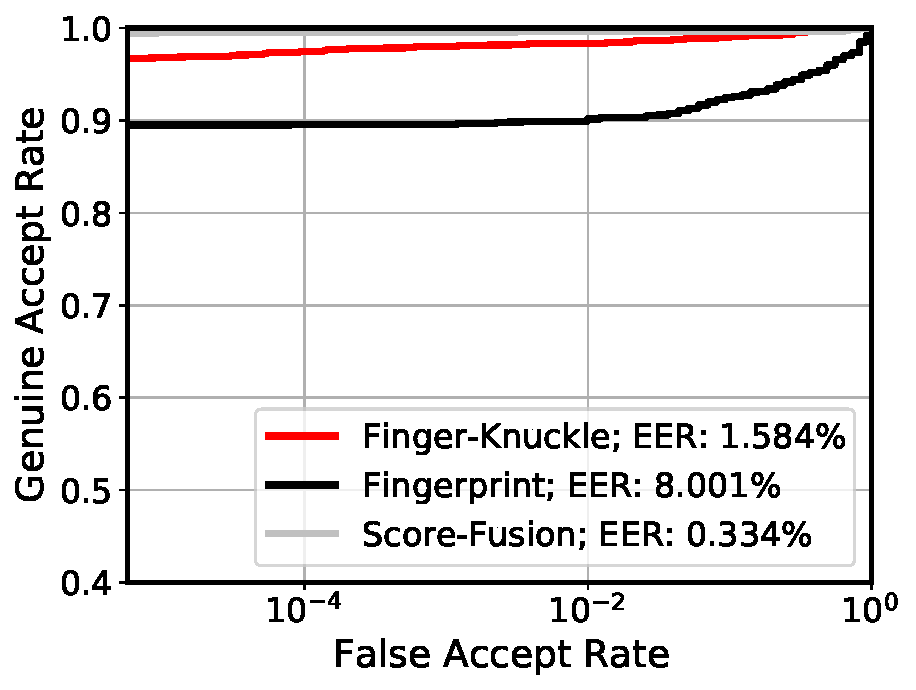
\includegraphics[width=2in]{Figure/09-12-2022/08(0.3-0.7).pdf}
        \label{}
    }
    \subfloat[]{
        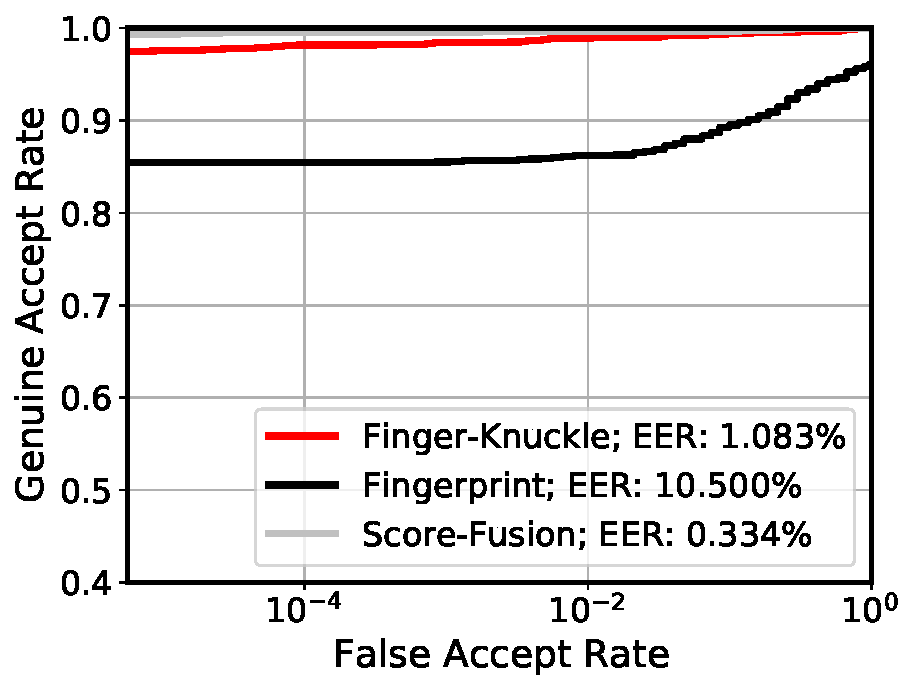
\includegraphics[width=2in]{Figure/09-12-2022/09(0.25-0.75).pdf}
        \label{}
    }
    \subfloat[]{
        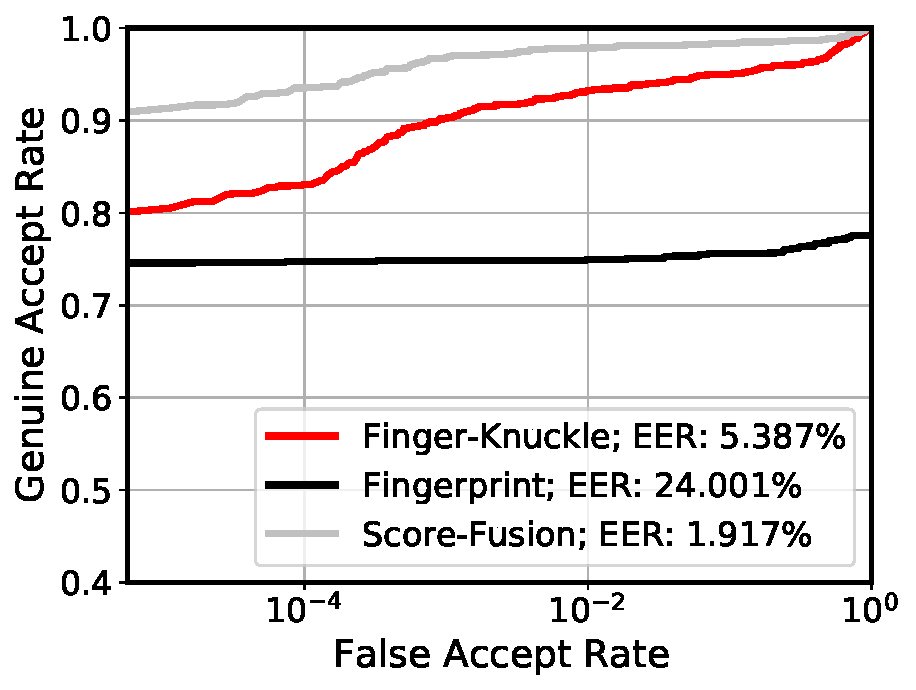
\includegraphics[width=2in]{Figure/09-12-2022/10(0.55-0.45).pdf}
        \label{}
    }

    \caption{Verification performance using holistic method to fusion finger knuckle and fingerprint matching score. (a) left little, (b) left ring, (c) left index, (d) left thumb, (e) right thumb, (f) right index, (g) right middle, (h) right ring, (i) right little.}
    \label{fusion-score}
\end{figure}
% \section{References}

\printbibliography[heading = none ]


\end{document}